\documentclass[letterpaper,10pt,serif,draftclsnofoot,onecolumn,compsoc,titlepage]{IEEEtran}

\usepackage{graphicx}                                        
\usepackage{amssymb}                                         
\usepackage{amsmath}                                         
\usepackage{amsthm}                                          
\usepackage{cite}
\usepackage{alltt}                                           
\usepackage{float}
\usepackage{color}
\usepackage{url}

\usepackage{balance}
\usepackage[TABBOTCAP, tight]{subfigure}
\usepackage{enumitem}

\usepackage{geometry}
\geometry{margin=.75in}
\usepackage{hyperref}
%\usetikzlibrary{shapes, positioning, calc}
\usepackage{caption}
\usepackage{listings}
%\usepackage[utf8]{inputenc}
%pull in the necessary preamble matter for pygments output

%% The following metadata will show up in the PDF properties
\hypersetup{
   colorlinks = true,
   citecolor = black,
   linkcolor = black,
   urlcolor = black,
   pdfauthor = {Shu-Ping Chien, Brock Smedley, and W Keith Striby Jr},
   pdfkeywords = {CS461 "Senior Project" Requirements Document},
   pdftitle = {CS 461 Requirements Document},
   pdfsubject = {CS 461 Requirements Document},
   pdfpagemode = UseNone
}

\parindent = 0.0 in
\parskip = 0.1 in
\title{Requirements Document: Multi-Camera, System-on-Chip (SoC) Based, Real-Time Video Processing for UAS and VR/AR Applications}
\author{Group 51: Shu-Ping Chien, Brock Smedley, and W Keith Stirby Jr \\ 03 November 2017 \\ CS-461, Senior Software Engineering Project, Fall 2017}
\begin{document}
\begin{titlepage}
\maketitle
\begin{abstract}

WRITE ME \\

\end{abstract}
\end{titlepage}
\newpage

\tableofcontents
\newpage

\section{Introduction}

\subsection{Purpose}

This software requirements specification is intended to define the requirements of the 
project of developing a multi-camera, multispectral image processing system, that 
operates on a System-on-Chip (SoC) at near-real-time, for use in ground and air based 
applications. Defined requirements will allow for a contract between us, the 
developers, and Rockwell Collins, our client, on what Rockwell Collins wants us to 
deliver in their desired software. This document is intended for review and reference 
by both the developers and the clients.\\

\subsection{Scope}

The product outlined in this requirements document will be the multi-camera, SoC based,
 real-time video processing for UAS and VR/AR applications. This product will need to 
 be able to generate a fused video output from a multi-camera input. The product is 
 intended to help initialize our client's development of a cheaper alternative to a 
 product that is already offered to their customers.\\

The software products that will be produced include software for a fused video output 
from the NVIDIA Jetson TX1 or TX2, receiving the input from two visible band cameras. 
The video output is expected to be near-real-time, and the latency from the camera 
input to the video output is expected to be improved upon throughout the project. Video 
input stretch goals is to have software that fuses the video output from the input of 
three, four, five, and six cameras, and have up to four infrared band inputs.\\ 

The goal of the software is to contribute to a project that will assist pilots during 
low visibility conditions during the day, night, and inclement weather for all phases 
of flight. The video input from infrared and visible band cameras combined with 
on-board sensor input, and databases will enhance a pilot vision for an unmanned and 
manned aerial vehicle.\\

\subsection{Definitions, Acronyms, Abbreviations}

...

\subsubsection{Definitions}

...

\subsubsection{Acronyms}

MAKE THIS INTO A TABLE\\
Term
Acronym\\
CSI
Camera Serial Interface\\
EVS
Enhanced Vision System\\
GPU
Graphic Processing Unit\\
ISP
Image Signal Processors\\
HUD
Head-up Display\\
SoC
System on a chip\\
SOM
System on a module\\
SWaP-C
Size, weight, power and cost\\
VI
Video Input\\
UAV
Unmanned Aerial Vehicle\\

\subsubsection{Abbreviations}

...

\subsection{References}

...

\subsection{Overview}

This project aims to create a device that is capable of combining the video input from 
two or more cameras and produce and output at near-real time. Our proposed solution 
will use an Nvidia Jetson device, which we will use for its integrated GPU.\\

We need this GPU to combine the images from multiple cameras. The end goal is to have 
a system that uses the input from multiple cameras that operate on different bands of 
the electromagnetic spectrum; infrared, ultraviolet, and visible light, among others. 
 By using these varying bands, we should be able to produce an image that can be used 
 to see in low-visibility situations, such as landing a UAV in fog.\\

The images we produce will be 2D representations of our collective image captures. In 
other words, we do not aim to create a 3D image or a dynamic focus image. This is 
certainly possible when using multiple cameras, but we simply aim to use multiple 
cameras on different spectral bands to create one image of one subject that is the 
combination of all images captured by the cameras.\\


\section{Overall Description}

\subsection{Product Perspective}

The system will consist of three parts: one Nvidia TX1/2, one CSI board, and at least 
two cameras. The cameras connect to the CSI board, which is connected to the Nvidia 
device. The Nvidia device is responsible for decoding the serial data retrieved by the 
CSI board from the cameras. The Nvidia device will then be used to execute the 
software for image processing and combining images from multiple cameras.\\

\begin{figure}[h]
    \centering
    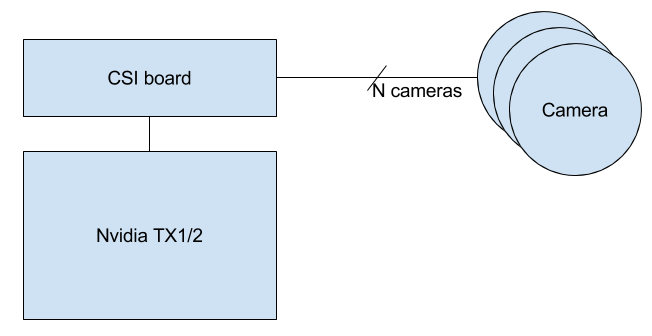
\includegraphics[width=1\textwidth]{diagram}
    \caption{System Diagram}
    \label{fig:mesh1}
\end{figure}

\subsection{Production Functions}

The EVS will be able to capture images from different spectral bands to create the 
clearest possible image in situations where visible light does not provide enough 
clarity. These images will be relayed in near-real time so that it can be used as a 
video feed. One use case would be for a pilot to be able to see the ground when landing 
in low-visibility conditions.\\

Since the EVS will be able to provide near to all weather operations, the images from 
the system will be analyzed and combined in several modes. The mode of equivalent 
vision can display images shot by cameras directly in normal visibilities condition 
such as clear daytime. The mode of synthetic vision will display images from the 
channels provide thermal images of the landscape and various types of lighting, for 
example incandescent, halogen, and LED lights, etcetera. Then the view on the display 
device will be real images combined with light structure.\\

\subsection{Constraints}

The system must operate in near-real time. In other words, the camera feed(s) must be 
processed quickly enough for the user to make snap decisions based on the feed. The 
NVIDIA board should process each frame before the next one arrives to be processed. 
If we’re recording at 30 frames per second (fps), then each output frame should be 
processed in less than 1/30 of a second.\\

\subsection{Assumptions \& Dependencies}

LIST ITEMS, WRONG, THIS SHOULD BE IN PARAGRAPH FORM\\
Software deployed on Nvidia TX1/2 with Nvidia Jetpack from Ubuntu machine
Adequate power supplies being used
Cameras being aimed at same subject; capturing mostly the same image
Each camera works independently of the system

\section{Specific Requirements}
THIS NEEDS TO BE IN PARAGRAPH FORM, WITH SECTIONS FROM THE IEEE STD 830-1998\\
\begin{enumerate}
	\item TX1/2
		\subitem Adequate power supply
		\subitem Nvidia Jetpack software + Ubuntu system to deploy it
	\item CSI Board
		\subitem Appropriate connectors
	\item Cameras
		\subitem Visible light
		\subitem Infrared
		\subitem UV
		\subitem ...
\end{enumerate}

\section{Development Schedule}

<Gantt Chart here>\\

\end{document}
